\documentclass[aspectratio=169, 10pt]{beamer}

% --- Theme & Styling ---
\usetheme{metropolis}
\usepackage{booktabs}
\usepackage{xspace}
\usepackage{tikz}
\usetikzlibrary{arrows.meta, positioning, shapes.geometric, calc}
\usepackage{listings}
\usepackage{tcolorbox}
\usepackage{graphicx}
\usepackage{caption}

% Caption styling for epigraphs below figures (consistent font, label, and centered alignment)
\captionsetup{font=scriptsize, labelfont=bf, textfont=it, skip=2pt, justification=centering}

% --- Color Palette ---
\definecolor{NavyDark}{HTML}{0F172A}
\definecolor{PrimaryBlue}{HTML}{1D4ED8}
\definecolor{TealDark}{HTML}{0F766E}
\definecolor{AmberWarm}{HTML}{B45309}
\definecolor{BgSlate}{HTML}{F8FAFC}
\definecolor{CodeSlate}{HTML}{1E293B}

\setbeamercolor{normal text}{fg=NavyDark, bg=white}
\setbeamercolor{alerted text}{fg=AmberWarm}
\setbeamercolor{example text}{fg=TealDark}
\setbeamercolor{progress bar}{fg=PrimaryBlue, bg=gray!25}
\setbeamercolor{title separator}{fg=PrimaryBlue}
\setbeamercolor{frametitle}{bg=NavyDark, fg=white}

% Metropolis tuning
\metroset{progressbar=frametitle, block=fill}

% --- Title Information ---
\title{Lab 1: Raw 8-Bit Ethernet Verification}
\subtitle{Hardware-in-the-Loop Simulation \& Waveform Analysis}
\date{\today}
\author{Zuñiga, Ivan Andrés}
\institute{Fundación Fulgor}

\begin{document}

% ==========================================
% SLIDE 1: Title Slide
% ==========================================
\maketitle

% ==========================================
% SLIDE 2: Testbench Architecture & Pipeline
% ==========================================
\begin{frame}{1. System Architecture \& Simulation Datapath}
\begin{columns}[c]
    \begin{column}{0.48\textwidth}
        \textbf{Hardware-in-the-Loop Setup:}
        \begin{itemize}\small
            \item \textbf{Host Interface}: \texttt{tap0} (\texttt{10.0.0.1/24}).
            \item \textbf{Target Interface}: \texttt{tap1} in namespace \texttt{ns\_b} (\texttt{10.0.0.2/24}).
            \item \textbf{C++ Testbench (\texttt{wrapper.cpp})}: Non-blocking TAP descriptor I/O streaming bytes to and from RTL.
            \item \textbf{RTL Core (\texttt{top.sv})}: Synchronous 8-bit bidirectional register datapath.
            \item \textbf{Framing}: Raw L2 frame stream, preamble and FCS handled at physical PHY layer.
        \end{itemize}
    \end{column}
    
    \begin{column}{0.50\textwidth}
        \begin{tcolorbox}[colback=BgSlate, colframe=PrimaryBlue, title=\footnotesize Dataflow Architecture, arc=2mm, top=1.5mm, bottom=1.5mm]
            \centering
            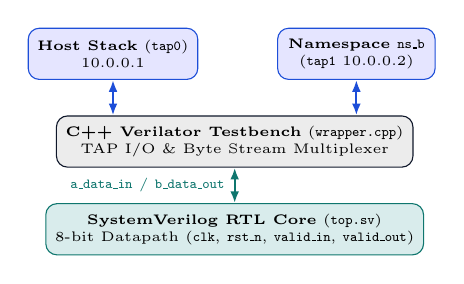
\begin{tikzpicture}[node distance=0.6cm, every node/.style={font=\tiny, align=center}]
                \node[draw=PrimaryBlue, fill=blue!10, rounded corners, minimum width=2.0cm, minimum height=0.65cm] (host) {\textbf{Host Stack} (\texttt{tap0})\\10.0.0.1};
                \node[draw=PrimaryBlue, fill=blue!10, rounded corners, minimum width=2.0cm, minimum height=0.65cm, right=1.0cm of host] (nsb) {\textbf{Namespace \texttt{ns\_b}}\\(\texttt{tap1} 10.0.0.2)};
                
                \node[draw=NavyDark, fill=gray!15, rounded corners, minimum width=4.4cm, minimum height=0.65cm, below=0.45cm of $(host.south)!0.5!(nsb.south)$] (wrap) {\textbf{C++ Verilator Testbench} (\texttt{wrapper.cpp})\\TAP I/O \& Byte Stream Multiplexer};
                
                \node[draw=TealDark, fill=teal!15, rounded corners, minimum width=4.4cm, minimum height=0.65cm, below=0.45cm of wrap] (rtl) {\textbf{SystemVerilog RTL Core} (\texttt{top.sv})\\8-bit Datapath (\texttt{clk}, \texttt{rst\_n}, \texttt{valid\_in}, \texttt{valid\_out})};
                
                % Arrows
                \draw[{Latex[length=1.5mm]}-{Latex[length=1.5mm]}, thick, color=PrimaryBlue] (host) -- (host |- wrap.north);
                \draw[{Latex[length=1.5mm]}-{Latex[length=1.5mm]}, thick, color=PrimaryBlue] (nsb) -- (nsb |- wrap.north);
                \draw[{Latex[length=1.5mm]}-{Latex[length=1.5mm]}, thick, color=TealDark] (wrap) -- node[left, font=\tiny]{\texttt{a\_data\_in} / \texttt{b\_data\_out}} (rtl);
            \end{tikzpicture}
        \end{tcolorbox}
        \vspace{1mm}
        \captionof{figure}{Simulation dataflow connecting Linux TAP interfaces to the SystemVerilog RTL core.}
    \end{column}
\end{columns}
\end{frame}

% ==========================================
% SLIDE 3: Environment Setup & Traffic Generation
% ==========================================
\begin{frame}{2. Environment Setup \& Traffic Generation}
\begin{columns}[c]
    \begin{column}{0.48\textwidth}
        \textbf{Execution Sequence:}
        \begin{enumerate}\footnotesize
            \item \textbf{TAP Network Initialization}:\\
            \texttt{sudo ./setup\_tap.sh}\\
            {\scriptsize Creates \texttt{tap0} and isolated namespace \texttt{ns\_b} with \texttt{tap1}.}
            
            \item \textbf{Verilator Build \& Run}:\\
            {\scriptsize\texttt{verilator --cc --trace --exe --build wrapper.cpp top.sv}}\\
            \texttt{sudo ./obj\_dir/emulator}
            
            \item \textbf{Packet Capture}:\\
            \texttt{sudo tcpdump -i tap0 -w lab1\_capture.pcap}
            
            \item \textbf{Pattern Traffic Injection}:\\
            \texttt{ping -c 2 -p cafe0001 -I tap0 10.0.0.2}
        \end{enumerate}
    \end{column}
    
    \begin{column}{0.50\textwidth}
        \centering
        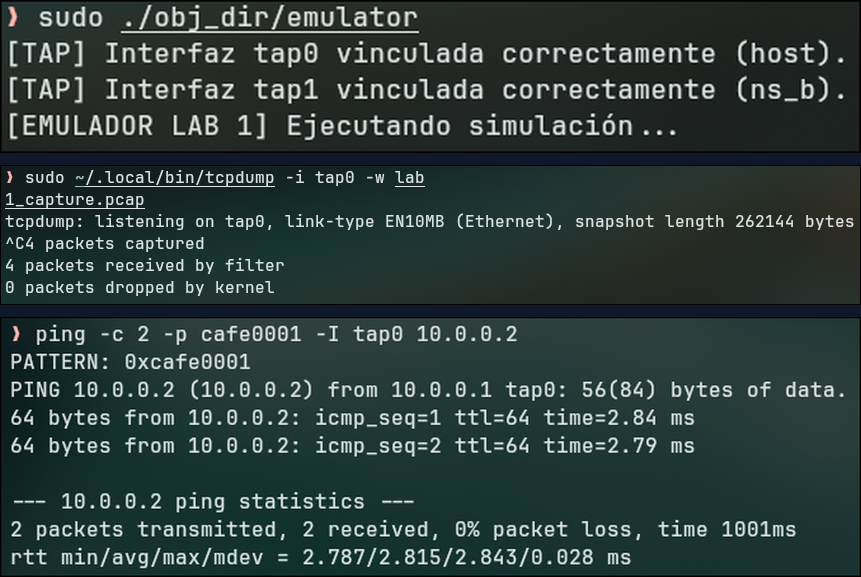
\includegraphics[width=\textwidth, height=0.68\textheight, keepaspectratio]{figures/screenshot1_terminal.png}
        \vspace{1mm}
        \captionof{figure}{Terminal execution showing TAP interface binding, Verilator build, and no loss in ICMP traffic.}
    \end{column}
\end{columns}
\end{frame}

% ==========================================
% SLIDE 4: Wireshark Packet Inspection
% ==========================================
\begin{frame}{3. Layer 2 / Layer 3 Wireshark Packet Analysis}
    \vspace{-2mm}
    \textbf{Captured ICMP Echo Request Frame (98 Bytes Total):}
    \begin{itemize}\scriptsize
        \item \textbf{Layer 2 Header (14B)}: Dst MAC \texttt{02:00:00:00:00:02}, Src MAC \texttt{02:00:00:00:00:01}, EtherType \texttt{0x0800} (IPv4).
        \item \textbf{Layer 3 Header (28B)}: IPv4 \texttt{10.0.0.1} $\rightarrow$ \texttt{10.0.0.2} (20B), ICMP Type 8 (Echo Request, Code 0, 8B).
        \item \textbf{Payload (56B)}: 16-byte kernel timestamp + 40-byte repeating pattern \texttt{ca fe 00 01}.
    \end{itemize}
    
    \vspace{2mm}
    \begin{center}
        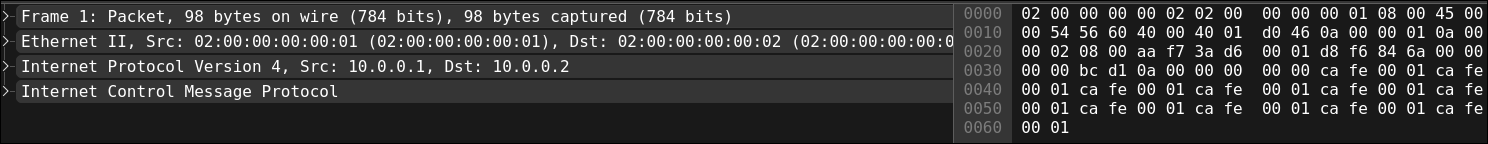
\includegraphics[width=0.98\textwidth, height=0.48\textheight, keepaspectratio]{figures/screenshot2_wireshark.png}
        \vspace{1mm}
        \captionof{figure}{Wireshark dissection and hex dump of the 98-byte captured ICMP Echo Request frame.}
    \end{center}
\end{frame}

% ==========================================
% SLIDE 5: SW-to-HW Correlation (Layer 2 Ethernet II)
% ==========================================
\begin{frame}{4. SW-to-HW Correlation: Layer 2 Header}
    \vspace{-2mm}
    \textbf{Ethernet II Header Stream Alignment (14 Bytes):}
    \begin{itemize}\scriptsize
        \item \textbf{Dst MAC (Bytes 0--5)}: \texttt{02 00 00 00 00 02} $\longleftrightarrow$ Clock Cycles 0--5 on \texttt{a\_data\_in[7:0]}.
        \item \textbf{Src MAC (Bytes 6--11)}: \texttt{02 00 00 00 00 01} $\longleftrightarrow$ Clock Cycles 6--11 on \texttt{a\_data\_in[7:0]}.
        \item \textbf{EtherType (Bytes 12--13)}: \texttt{08 00} (IPv4) $\longleftrightarrow$ Clock Cycles 12--13 on \texttt{a\_data\_in[7:0]}.
    \end{itemize}
    
    \vspace{2mm}
    \begin{center}
        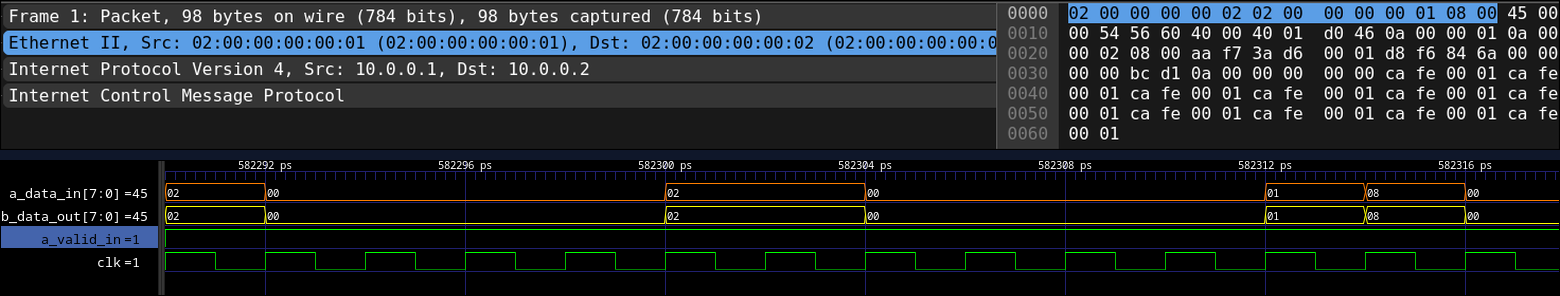
\includegraphics[width=0.98\textwidth, height=0.48\textheight, keepaspectratio]{figures/screenshot3_correlation.png}
        \vspace{1mm}
        \captionof{figure}{Cycle-by-cycle alignment between Wireshark Layer 2 hex dump and GTKWave signal transitions.}
    \end{center}
\end{frame}

% ==========================================
% SLIDE 6: SW-to-HW Correlation (Layer 3 IPv4)
% ==========================================
\begin{frame}{5. SW-to-HW Correlation: Layer 3 IPv4 Header}
    \vspace{-2mm}
    \textbf{IPv4 Header Stream Alignment (20 Bytes):}
    \begin{itemize}\scriptsize
        \item \textbf{Version / IHL / Length (Bytes 14--17)}: \texttt{45 00 00 54} (IPv4, 20B Header, 84B Total) $\longleftrightarrow$ Clock Cycles 14--17.
        \item \textbf{ID / Flags / TTL / Proto (Bytes 18--23)}: \texttt{56 60 40 00 40 01} (TTL 64, ICMP Proto 1) $\longleftrightarrow$ Clock Cycles 18--23.
        \item \textbf{Checksum / IP Endpoints (Bytes 24--33)}: \texttt{D0 46} (Checksum), \texttt{0A 00 00 01} (Src), \texttt{0A 00 00 02} (Dst) $\longleftrightarrow$ Cycles 24--33.
    \end{itemize}
    
    \vspace{2mm}
    \begin{center}
        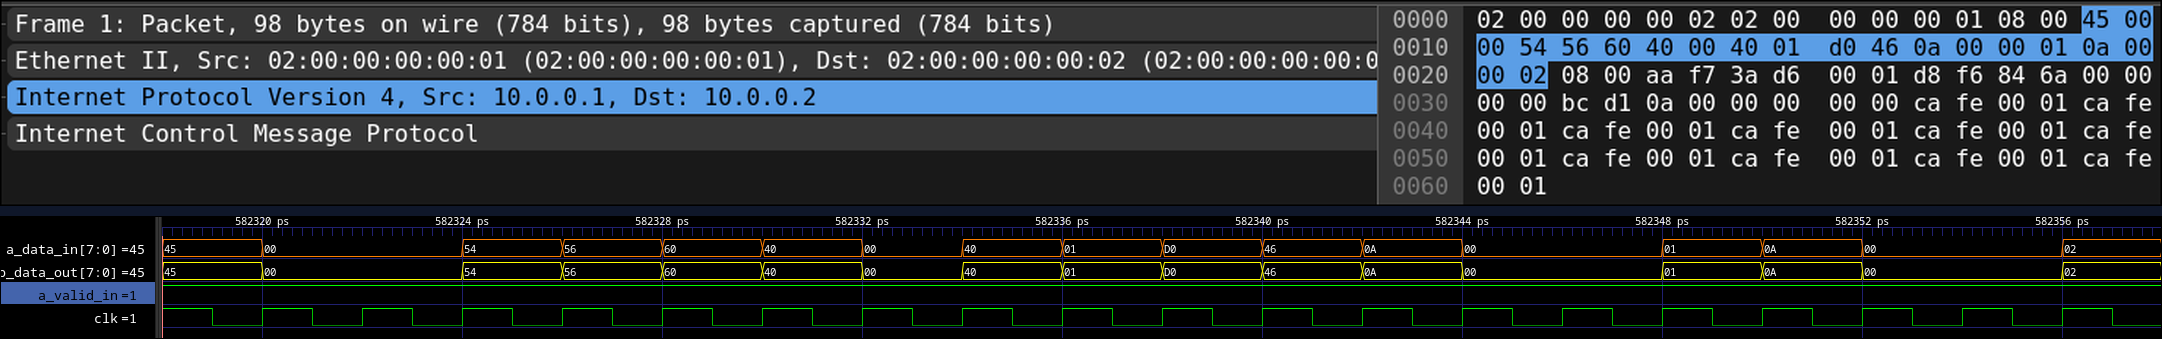
\includegraphics[width=0.98\textwidth, height=0.48\textheight, keepaspectratio]{figures/screenshot3_ipv4_correlation.png}
        \vspace{1mm}
        \captionof{figure}{Cycle-by-cycle hardware bus matching for the 20-byte IPv4 packet header stream.}
    \end{center}
\end{frame}

% ==========================================
% SLIDE 7: SW-to-HW Correlation (Layer 3 ICMP & Payload)
% ==========================================
\begin{frame}{6. SW-to-HW Correlation: ICMP \& Payload}
    \vspace{-2mm}
    \textbf{ICMP Header \& Payload Stream Alignment (64 Bytes):}
    \begin{itemize}\scriptsize
        \item \textbf{ICMP Header (Bytes 34--41)}: \texttt{08 00 AA F7 3A D6 00 01} (Type 8, Code 0, Checksum, ID, Seq) $\longleftrightarrow$ Clock Cycles 34--41.
        \item \textbf{Timestamp Data (Bytes 42--57)}: \texttt{D8 F6 84 6A ... BC D1 0A 00 ...} $\longleftrightarrow$ Clock Cycles 42--57.
        \item \textbf{Custom Payload Pattern (Bytes 58--97)}: Repeating signature \texttt{CA FE 00 01} $\longleftrightarrow$ Clock Cycles 58+ on \texttt{a\_data\_in[7:0]}.
    \end{itemize}
    
    \vspace{2mm}
    \begin{center}
        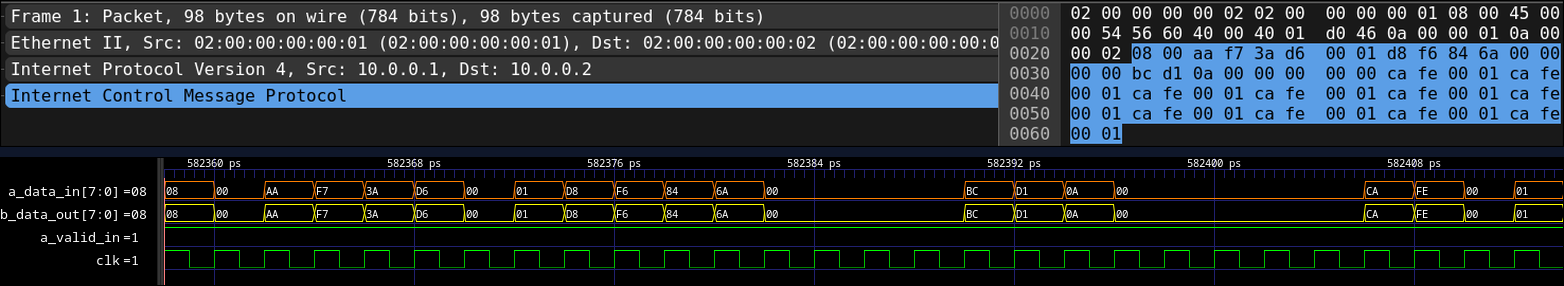
\includegraphics[width=0.98\textwidth, height=0.48\textheight, keepaspectratio]{figures/screenshot3_icmp_correlation.png}
        \vspace{1mm}
        \captionof{figure}{Hardware bus streaming of the ICMP header and custom \texttt{0xCAFE0001} repeating payload pattern.}
    \end{center}
\end{frame}

% ==========================================
% SLIDE 8: Pipeline Latency & Cycle Delay Analysis
% ==========================================
\begin{frame}{7. Pipeline Latency \& Cycle Delay Analysis}
    \vspace{-2mm}
    \textbf{RTL Registered Datapath Verification (\texttt{top.sv}):}
    \begin{itemize}\scriptsize
        \item \textbf{Setup Phase (\texttt{clk=0})}: Input byte \texttt{a\_data\_in = 0x02} and \texttt{a\_valid\_in = 1'b1} are driven during the posedge.
        \item \textbf{Clock Edge Latch (\texttt{clk=1})}: Output valid \texttt{b\_valid\_out} and data \texttt{b\_data\_out = 0x02} assert on the rising edge.
        \item \textbf{1-Cycle Latency}: \texttt{wrapper.cpp} drives inputs on \texttt{clk=0} to model the setup window for RTL non-blocking assignments (\texttt{<=}), giving a 1-clock delay ($T_{\text{latency}} = 1\ T_{\text{clk}}$) through the D-FF register stage.
    \end{itemize}
    
    \vspace{2mm}
    \begin{center}
        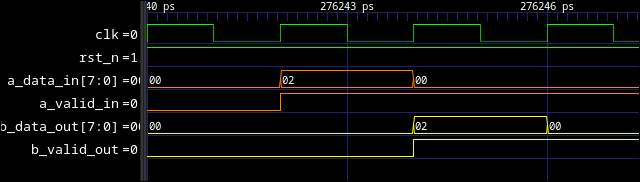
\includegraphics[width=0.98\textwidth, height=0.48\textheight, keepaspectratio]{figures/screenshot5_latency.png}
        \vspace{1mm}
        \captionof{figure}{GTKWave cycle zoom displaying the exact 1-clock-cycle delay between input assertion and registered output valid.}
    \end{center}
\end{frame}

% ==========================================
% SLIDE 9: Conclusion / Thank You
% ==========================================
\begin{frame}[standout]
    \Huge \textbf{Thank You!}\\[1.2em]
\end{frame}

\end{document}
